% BLM308 Veri Madenciliği Final Projesi - LaTeX Raporu
\documentclass[12pt,a4paper]{report}

\usepackage[utf8]{inputenc}
\usepackage[T1]{fontenc}
\usepackage[turkish]{babel}
\usepackage{geometry}
\geometry{margin=2.5cm}
\usepackage{graphicx}
\usepackage{booktabs}
\usepackage{hyperref}
\usepackage{float}
\usepackage{caption}
\usepackage{subcaption}
\usepackage{enumitem}
\usepackage{setspace}
\onehalfspacing

\hypersetup{
    colorlinks=true,
    linkcolor=blue,
    citecolor=blue,
    urlcolor=blue
}

\graphicspath{{../reports/figures/}}

\title{%
    \textbf{BLM308 Veri Madenciliği Final Projesi}\\[0.4cm]
  \Large Çevrimiçi Alışveriş Ürün İade Tahmini
}
\author{Emre Kaya\\Öğrenci No: 231041045\\BLM308 Veri Madenciliği\\Teslim: Mayıs 2026\\\url{https://github.com/emrekayy/blm308-urun-iade-tahmini}}
\date{}

\begin{document}

\maketitle
\tableofcontents
\newpage

\chapter*{Öğrenci Bilgileri}
\addcontentsline{toc}{chapter}{Öğrenci Bilgileri}
\begin{itemize}
    \item Ad Soyad: Emre Kaya
    \item Öğrenci Numarası: 231041045
    \item Ders: BLM308 Veri Madenciliği
    \item Teslim Tarihi: Mayıs 2026
    \item GitHub Deposu: \url{https://github.com/emrekayy/blm308-urun-iade-tahmini}
\end{itemize}

\chapter*{Proje Görev Dağılımı}
\addcontentsline{toc}{chapter}{Proje Görev Dağılımı}
Bu proje bireysel olarak Emre Kaya tarafından gerçekleştirilmiştir. Veri ön işleme, keşifsel veri analizi, model eğitimi, değerlendirme, rapor ve sunum hazırlığının tamamı proje sahibi tarafından yapılmıştır.

\chapter*{Özet}
\addcontentsline{toc}{chapter}{Özet}
Bu proje, bir e-ticaret siparişinin iade edilip edilmeyeceğini tahmin eden ikili sınıflandırma problemini ele almaktadır.
\texttt{product\_return\_prediction.csv} veri seti (1.500 kayıt) kullanılarak CRISP-DM metodolojisi uygulanmış, keşifsel veri analizi gerçekleştirilmiş ve beş sınıflandırma algoritması eğitim kümesi üzerinde 10 katmanlı stratified çapraz doğrulama ile karşılaştırılmıştır.
En iyi performansı gösteren model Random Forest olmuş; ayrılmış test kümesinde yalnızca bir kez değerlendirilmiş ve F1-skoru 0,2206, ROC-AUC değeri 0,4793 elde edilmiştir.

\chapter{Problem Tanımı}
Ürün iadeleri çevrimiçi perakendede operasyonel maliyet, stok yönetimi sorunları ve müşteri memnuniyetsizliği yaratmaktadır.
Bu projenin amacı, \texttt{return\_status} (0 = iade edilmedi, 1 = iade edildi) değişkenini tahmin ederek perakendecilerin kalite kontrolünü önceliklendirmesine, fiyatlandırma politikalarını düzenlemesine ve müşteri deneyimini iyileştirmesine yardımcı olmaktır.

\chapter{Motivasyon ve İş Değeri}
\begin{itemize}
    \item Yüksek riskli siparişleri erken tespit ederek ters lojistik maliyetlerini azaltmak
    \item İade edilecek ürünleri öngörerek envanter planlamasını iyileştirmek
    \item Düşük puanlı alışverişlerde hedefli müşteri hizmeti sunmak
    \item Veriye dayalı fiyatlandırma ve ürün portföyü kararlarını desteklemek
\end{itemize}

\chapter{İlgili Çalışmalar / Literatür}
E-ticaret analitiğinde iade tahmini; müşteri davranışı, ürün özellikleri ve satın alma sonrası geri bildirimler kullanılarak incelenmiştir.
Önceki çalışmalar, fiyat duyarlılığı, ürün kalitesi sinyalleri (puanlar) ve ürüne özgü kalıpların iadeler için güçlü öngörücüler olduğunu göstermektedir.
Dengesiz perakende sınıflandırma görevlerinde ağaç tabanlı topluluk modelleri ve lojistik regresyon yaygın olarak kullanılan temel yöntemlerdir.

\chapter{CRISP-DM Metodolojisi}
\begin{enumerate}
    \item \textbf{İş Anlayışı:} İade tahminini maliyet azaltma odaklı bir kullanım senaryosu olarak tanımlama
    \item \textbf{Veri Anlayışı:} Şema, eksik değerler ve sınıf dengesizliğini inceleme
    \item \textbf{Veri Hazırlığı:} Ürün encoding, ölçekleme, stratified bölünme
    \item \textbf{Modelleme:} Decision Tree, Random Forest, Logistic Regression, Naive Bayes, KNN
    \item \textbf{Değerlendirme:} Eğitim kümesinde 10 katmanlı stratified CV; test kümesi yalnızca final değerlendirme
    \item \textbf{Dağıtım:} Perakende operasyonları için uygulanabilir içgörülerin dokümante edilmesi
\end{enumerate}

\chapter{Veri Seti Kaynağı ve Açıklaması}
\begin{itemize}
    \item \textbf{Dosya:} \texttt{product\_return\_prediction.csv}
    \item \textbf{Kayıt sayısı:} 1.500 gözlem, 5 sütun
    \item \textbf{Sütunlar:} \texttt{order\_id}, \texttt{product\_id}, \texttt{price}, \texttt{rating}, \texttt{return\_status}
    \item \textbf{Hedef:} \texttt{return\_status} (Sınıf 0: 1.094, Sınıf 1: 406)
    \item \textbf{Eksik değer:} Yok
    \item \textbf{Eksik sütunlar:} Kategori, indirim, teslimat süresi bulunmamaktadır
\end{itemize}

\chapter{Keşifsel Veri Analizi (EDA)}
Sınıf dağılımı, fiyat-iade ilişkisi, puan dağılımı ve korelasyon grafikleri oluşturulmuştur.
Kategori, indirim ve teslimat süresi grafikleri veri setinde ilgili sütunlar olmadığı için atlanmıştır.

\begin{figure}[H]
    \centering
    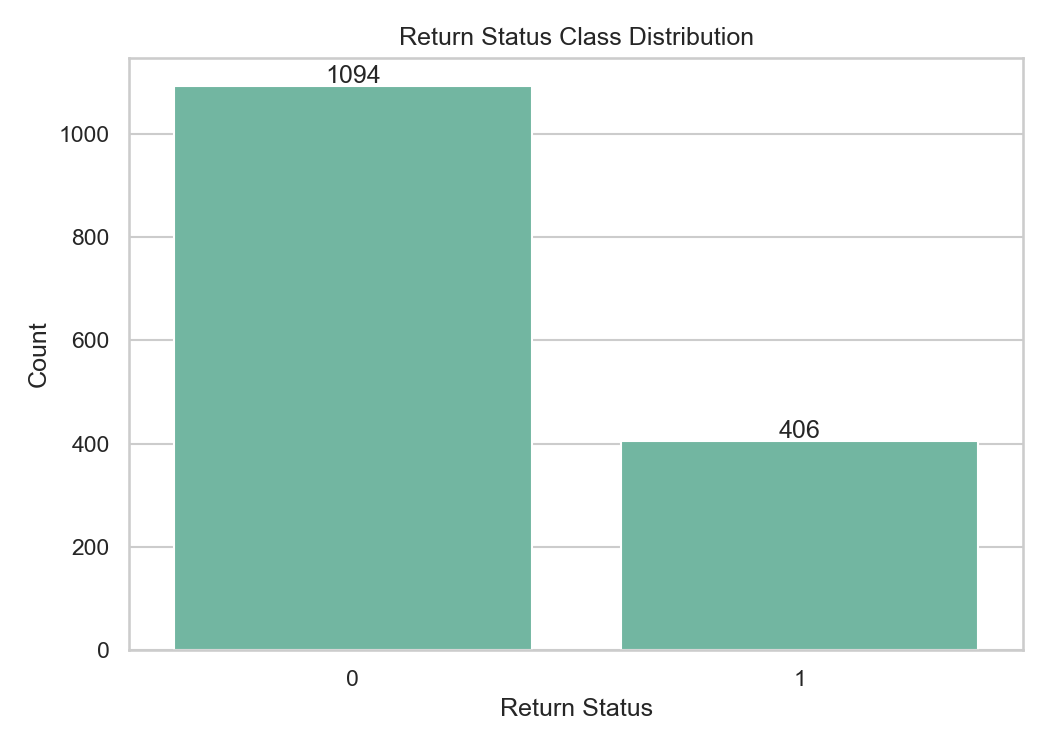
\includegraphics[width=0.75\textwidth]{01_class_distribution.png}
    \caption{Sınıf dağılımı (iade oranı $\approx$ \%27)}
\end{figure}

\begin{figure}[H]
    \centering
    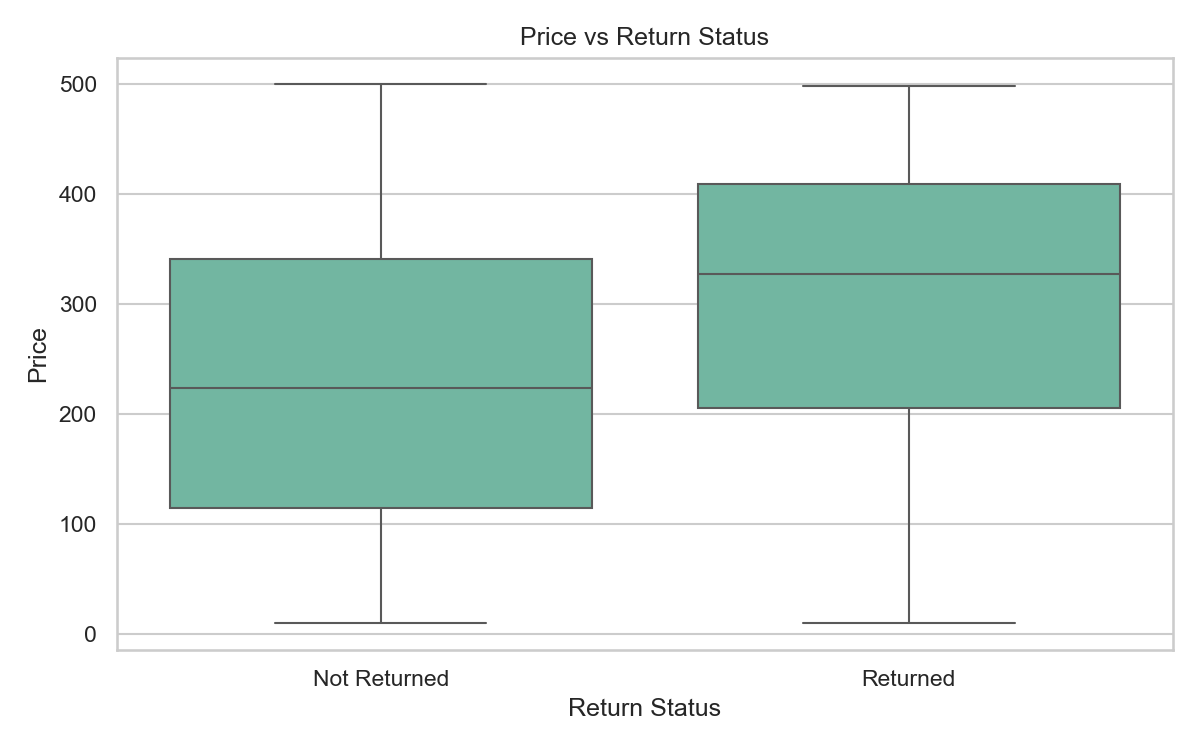
\includegraphics[width=0.8\textwidth]{03_price_vs_return.png}
    \caption{Fiyat ve iade durumu ilişkisi}
\end{figure}

\begin{figure}[H]
    \centering
    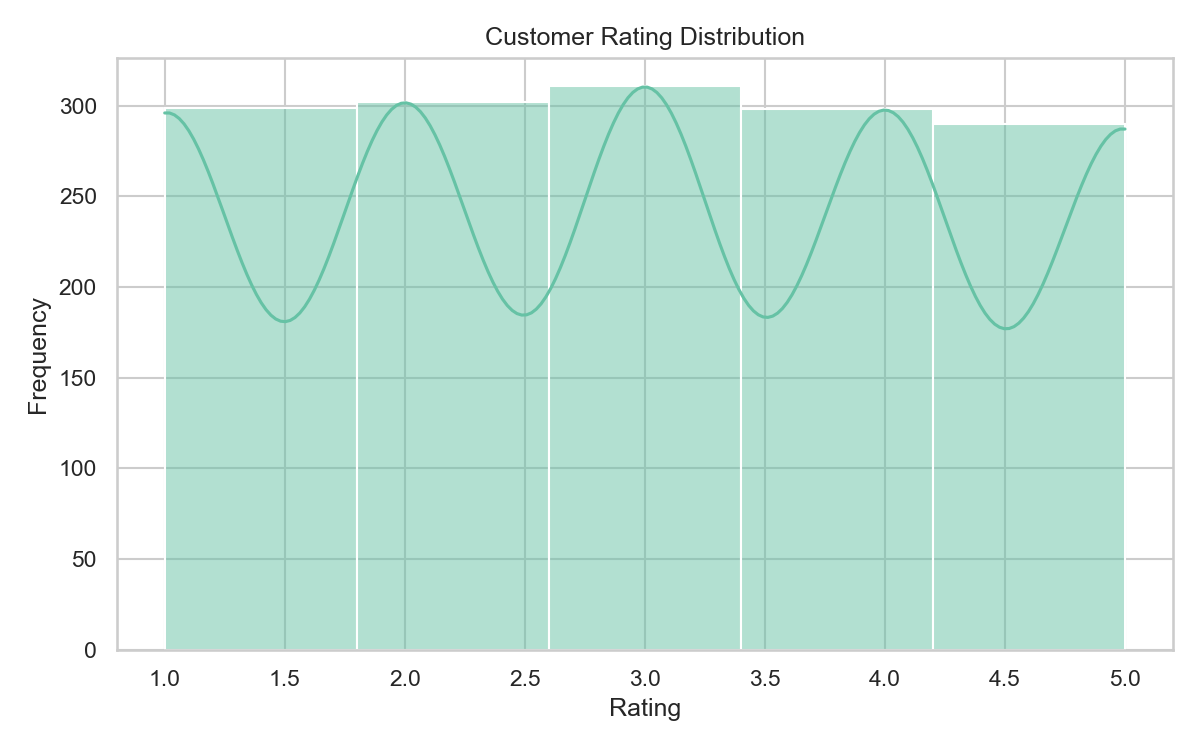
\includegraphics[width=0.8\textwidth]{05_rating_distribution.png}
    \caption{Müşteri puanı dağılımı}
\end{figure}

\begin{figure}[H]
    \centering
    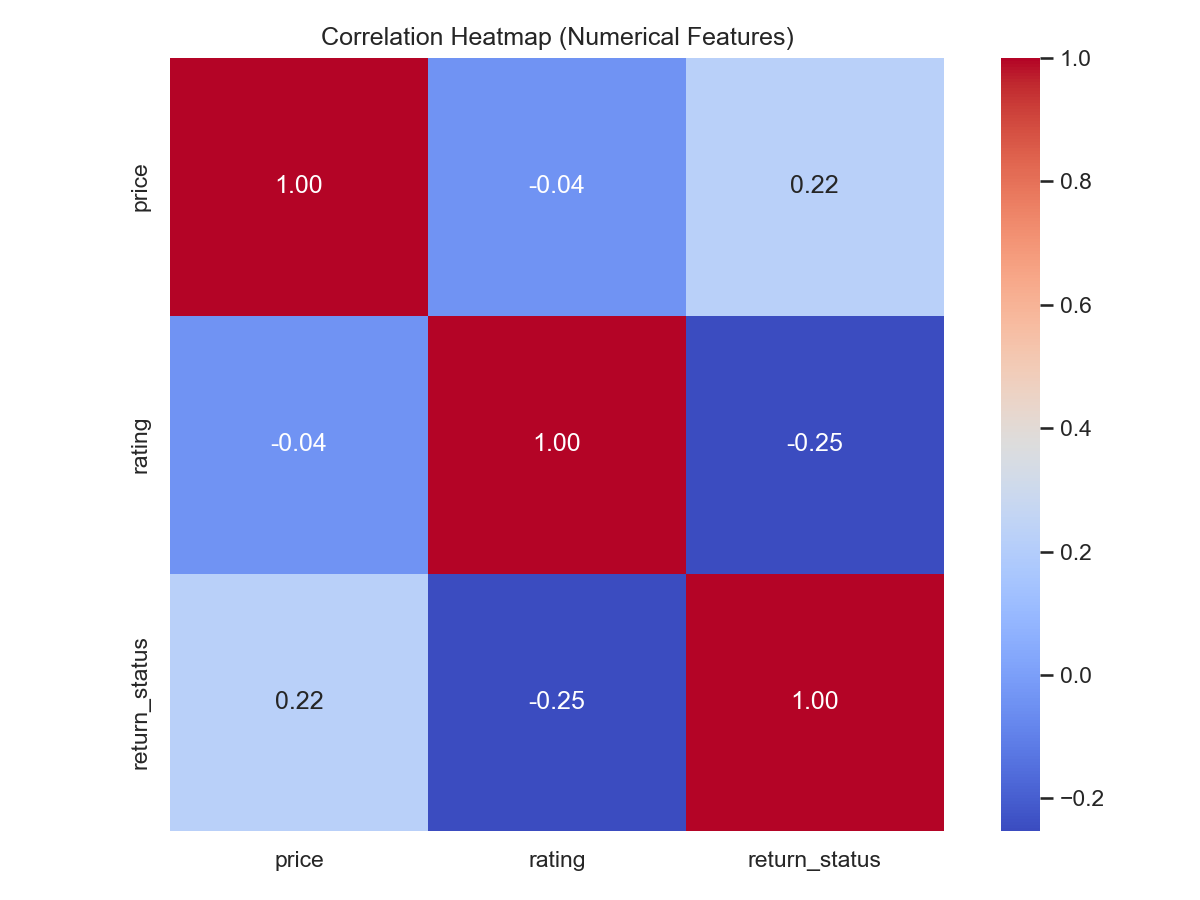
\includegraphics[width=0.75\textwidth]{07_correlation_heatmap.png}
    \caption{Sayısal özellikler korelasyon ısı haritası}
\end{figure}

\chapter{Ön İşleme Adımları}
\begin{itemize}
    \item \texttt{order\_id} benzersiz tanımlayıcı olarak çıkarıldı
    \item \texttt{product\_id} ordinal özellik olarak kullanılmadı; Label Encoding kaldırıldı
    \item \texttt{product\_id\_frequency}: her ürünün yalnızca eğitim kümesindeki görülme sayısı
    \item \texttt{product\_return\_rate}: ürün bazlı iade oranı yalnızca eğitim kümesinden hesaplandı
    \item Eğitimde görülmeyen 78 test ürünü için frekans=0, iade oranı=eğitim ortalaması (0,2708)
    \item \texttt{price}, \texttt{rating} ve türetilen özelliklere StandardScaler (yalnızca eğitimde fit)
    \item Stratified \%80/\%20 bölünme encoding öncesinde yapıldı (\texttt{random\_state=42})
\end{itemize}

\chapter{Seçilen Modeller}
\begin{itemize}
    \item Decision Tree (Karar Ağacı) --- \texttt{max\_depth=8}, \texttt{min\_samples\_leaf=5}
    \item Random Forest (Rastgele Orman) --- \texttt{n\_estimators=200}, \texttt{max\_depth=12}
    \item Logistic Regression (Lojistik Regresyon) --- \texttt{max\_iter=1000}
    \item Gaussian Naive Bayes
    \item K-Nearest Neighbors (KNN) --- \texttt{n\_neighbors=7}
\end{itemize}

\chapter{Değerlendirme Kurulumu}
Veri seti stratified \%80/\%20 oranında eğitim (1.200) ve test (300) kümelerine ayrılmıştır.
\texttt{product\_id} için frekans ve iade oranı özellikleri yalnızca eğitim kümesinden türetilmiştir.
Çapraz doğrulama sırasında bu özellikler \textbf{her fold içinde yeniden hesaplanarak} target leakage önlenmiştir.
Model karşılaştırması yalnızca eğitim kümesi üzerinde 10 katmanlı Stratified Cross Validation ile yapılmıştır.
Test kümesi modele hiçbir aşamada dahil edilmemiş; yalnızca seçilen en iyi model tam eğitim kümesi ile eğitildikten sonra \textbf{bir kez} final değerlendirme için kullanılmıştır.
Model seçim kriteri: çapraz doğrulama ortalama F1-skoru.

\chapter{Performans Karşılaştırması}
Aşağıdaki tablo yalnızca eğitim kümesi üzerindeki 10 katmanlı CV ortalamalarını göstermektedir.

\begin{table}[H]
    \centering
    \caption{Model performans karşılaştırması (10-fold Stratified CV, eğitim kümesi)}
    \begin{tabular}{lccccc}
        \toprule
        Model & Doğruluk & Kesinlik & Duyarlılık & F1-Skoru & ROC-AUC \\
        \midrule
        Random Forest       & 0,6717 & 0,3551 & 0,2734 & \textbf{0,3065} & 0,5333 \\
        Decision Tree       & 0,6275 & 0,2960 & 0,2733 & 0,2822 & 0,5172 \\
        Naive Bayes         & 0,6633 & 0,3303 & 0,2455 & 0,2791 & 0,5766 \\
        KNN                 & 0,6692 & 0,3299 & 0,2269 & 0,2663 & 0,5199 \\
        Logistic Regression & 0,6683 & 0,3270 & 0,2270 & 0,2646 & 0,5713 \\
        \bottomrule
    \end{tabular}
\end{table}

\chapter{En İyi Model Sonuçları}
Eğitim kümesi CV F1-skoruna göre seçilen en iyi model: \textbf{Random Forest}.

Seçilen model tam eğitim kümesi (1.200 kayıt) ile eğitilmiş ve test kümesi (300 kayıt) üzerinde yalnızca bir kez değerlendirilmiştir.

\begin{table}[H]
    \centering
    \caption{Random Forest --- bağımsız test kümesi metrikleri}
    \begin{tabular}{lc}
        \toprule
        Metrik & Değer \\
        \midrule
        Doğruluk  & 0,6467 \\
        Kesinlik  & 0,2727 \\
        Duyarlılık & 0,1852 \\
        F1-skoru  & 0,2206 \\
        ROC-AUC   & 0,4793 \\
        \bottomrule
    \end{tabular}
\end{table}

Confusion matrix (test): TN=179, FP=40, FN=66, TP=15.

\begin{figure}[H]
    \centering
    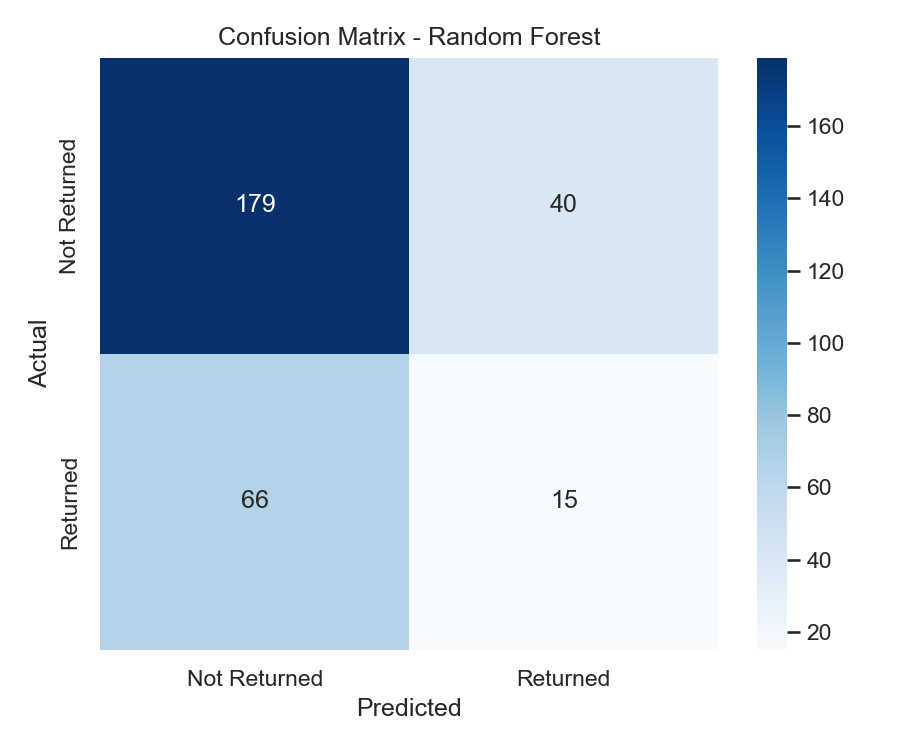
\includegraphics[width=0.65\textwidth]{08_confusion_matrix_best_model.png}
    \caption{En iyi model için karmaşıklık matrisi (Random Forest, test kümesi)}
\end{figure}

\begin{figure}[H]
    \centering
    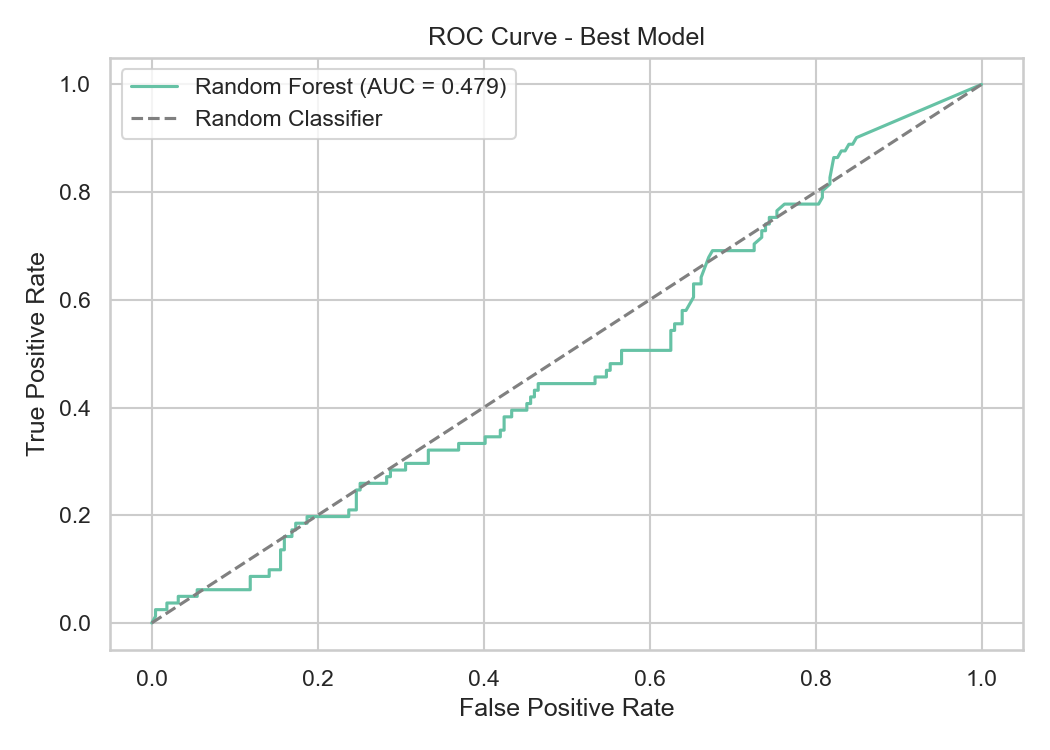
\includegraphics[width=0.75\textwidth]{09_roc_curve_best_model.png}
    \caption{En iyi model için ROC eğrisi (test kümesi)}
\end{figure}

\begin{figure}[H]
    \centering
    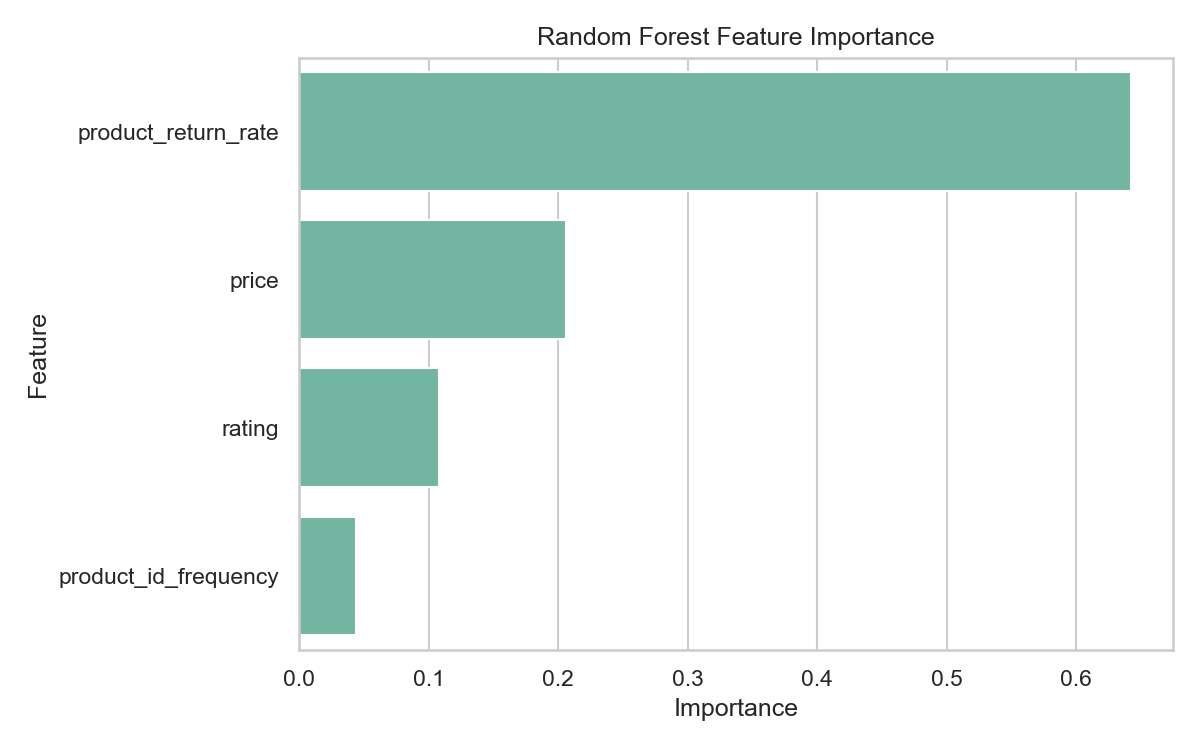
\includegraphics[width=0.8\textwidth]{10_feature_importance_random_forest.png}
    \caption{Random Forest özellik önem dereceleri}
\end{figure}

\chapter{Önyargı-Varyans Tartışması}
Karar Ağacı modelleri daha yüksek varyansa sahip olabilir ve gürültülü kalıplara aşırı uyum gösterebilir.
Random Forest varyansı azaltır ancak ürün düzeyindeki kalıpları ezberleyebilir.
Lojistik Regresyon daha düşük varyans sunar fakat doğrusal olmayan etkileşimleri yakalayamayabilir.
Seçilen model, genelleme ile tahmin performansı arasında denge kurmayı hedefler.

\chapter{İş Yorumu}
Düşük müşteri puanları ve ürün bazlı iade oranı sinyalleri önemli öngörücülerdir.
Perakende ekipleri iade risk skorlarını proaktif destek, kalite incelemesi ve fiyatlandırma gözden geçirmesi için kullanabilir.

\chapter{Kısıtlamalar}
\begin{itemize}
    \item Sınırlı özellik seti (demografi, kategori, indirim, teslimat yok)
    \item Sınıf dengesizliği azınlık sınıfının duyarlılığını olumsuz etkiler
    \item Test kümesinde 78 eğitimde görülmemiş ürün bulunmaktadır
    \item Sonuçlar geçmiş verilere dayanır; mevsimsel etkiler yansıtılmayabilir
\end{itemize}

\chapter{Gelecek Çalışmalar}
\begin{itemize}
    \item Yorum metinleri, teslimat süresi ve promosyon verilerinin entegrasyonu
    \item SMOTE veya maliyet-duyarlı öğrenme ile sınıf dengesizliği yönetimi
    \item Ürün embedding yöntemleri
    \item Gerçek zamanlı skorlama API'si
\end{itemize}

\chapter{Yapay Zeka Kullanım Beyanı}
Proje yapılırken yapay zeka araçlarından yararlanılmıştır.

\begin{thebibliography}{9}
\bibitem{crispdm}
Chapman, P. et al. (2000). \textit{CRISP-DM 1.0 Step-by-step data mining guide}.

\bibitem{rf}
Breiman, L. (2001). Random Forests. \textit{Machine Learning}, 45(1), 5--32.

\bibitem{sklearn}
Pedregosa, F. et al. (2011). Scikit-learn: Machine Learning in Python.
\end{thebibliography}

\end{document}
